\subsection{Robot Operating System}
The Robot Operating System (ROS) was developed by Willow Garage,  originally
for  the  PR2  robot  in  2007  [Quigley et al., 2009].   It  is  an  open  source  framework
for  developing  software  in  robotics  with  a  focus  on  the  ability  to  run  parallel  on
distributed  computer  systems.   It  can  be  run  on  different  operating  systems,  but
only Ubuntu and Debian are officially supported.  Its main advantage is a big library
of  available  software  modules  for  common  robotics  tasks.   These  are  developed,
maintained and documented by the ROS community and adding further modules is
easy.  Using ROS decreases the time for developing software as most of the parts can
be taken from the library.  In the following section, a short overview of the concepts
of ROS is provided.  A deeper insight can be found in the online documentation [3].

\subsubsection*{Nodes}
A node is a process in the ROS system.  It can communicate with other ROS nodes
via  topics  or  services.   In  doing  so,  all  nodes  form  a  computational  graph.   Each
node has typically a clearly defined subtask.  For example one node gets the camera
image, a second node detects balls on this image, and a third node computes the
ball positions.  Nodes can be easily reused in different tasks, for example the node
which gets the camera image can be reused in a different task that detects goals.
Open  source  implementations  of  nodes  for  most  standard  subtasks,  especially
hardware controlling, already exist.  Thereby the effort in implementing a new task
is drastically decreased.  The most important packages used for this thesis are men-
tioned in section 2.3.7

\begin{figure}[htbp]
    \centering
    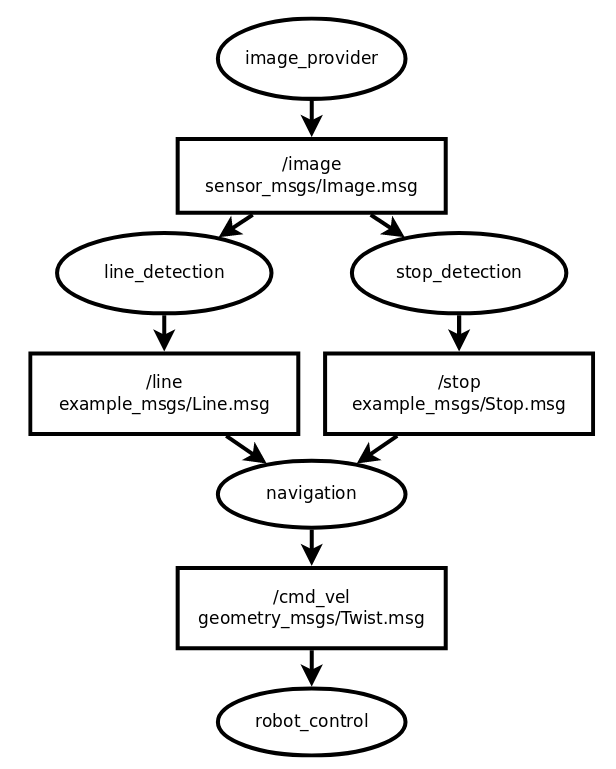
\includegraphics[width=0.6\textwidth]{chapter2/images/example_ros.png}
    \caption{ตัวอย่างสถาปัตยกรรมของ ROS}
    \label{fig:poppy_humanoid}
\end{figure}

Example ROS architecture for a simple wheeled robot with the task to
follow  a  line  until  it  finds  a  stop  marker.   The  nodes  are  displayed  as
ellipses with a name and the topics are shown as rectangles with name
and message type.  First, an image is provided from the camera.  Lines
and stop markers are detected on this image.  Based on this information,
a navigation node computes the necessary movement of the robot and
publishes it.  The robot
control node is then controlling the motors of
the robot accordingly
\begin{figure}[htbp]
    \centering
    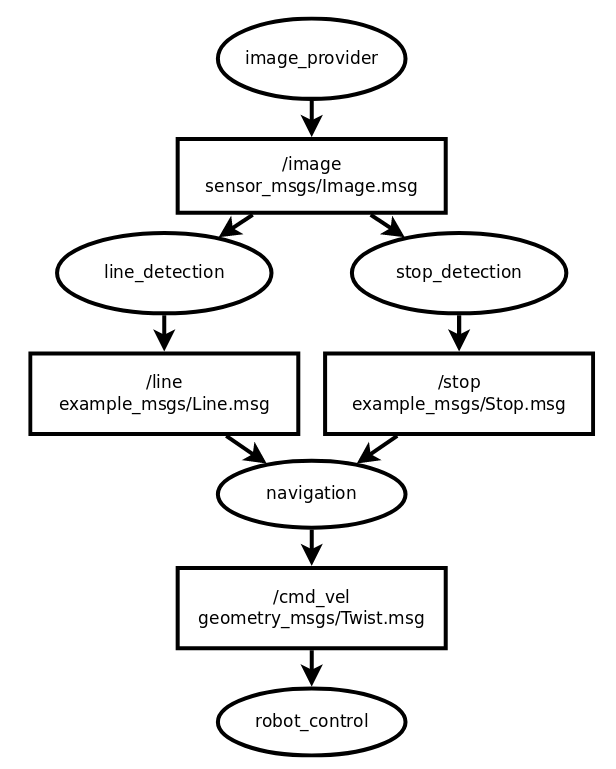
\includegraphics[width=0.6\textwidth]{chapter2/images/example_ros.png}
    \caption{ตัวอย่างสถาปัตยกรรมของ ROS}
    \label{fig:poppy_humanoid}
\end{figure}


\begin{table}[htbp]
	\begin{subtable}[h]{0.40\textwidth}
		\centering
		\begin{tabular}{| p{4cm}| p{1.5cm} |}
            \hline 
            \multicolumn{2}{|c|}{Twist.msg} \\
            \hline
			geometry\_msgs/Vector3 & linear \\
			geometry\_msgs/Vector3 & angular \\
            \hline  
		\end{tabular}
		\caption{First Week}
		\label{tab:week1}
	\end{subtable}
	\hfill
	\begin{subtable}[h]{0.40\textwidth}
		\centering
		\begin{tabular}{| p{1.5cm}| p{2.5cm} |}
            \hline 
            \multicolumn{2}{|c|}{Stop.msg} \\
            \hline
			uint8 & RED = 0 \\
            uint8 & GREEN = 1 \\
            uint8 & color \\
            float32 & distance \\
            \hline  
		\end{tabular}
		\caption{First Week}
		\label{tab:week1}
	\end{subtable}
	\caption{Max and min temps recorded in the first two weeks of July}
	\label{tab:temps}
\end{table}

